\chapter{Vehicle Telematics and Task Definition}
\label{sec:task-definition}

\section{Tesla EV Telematics Dataset}
\label{sec:dataset}

The primary experimental setting is the Tesla electric-vehicle use case in the
supervisor-provided notebook and the corresponding repository-local result
directory \path{results/tesla_ev_graph_recovery}. The repository also contains
a local CSV copy at \path{data/tesla.csv}. This file contains 65,261 telemetry
rows and eight source columns:
\texttt{timestamp}, \texttt{electricenergyremaining},
\texttt{electricremaining}, \texttt{speed\_kmh},
\texttt{acceleration\_kmh2}, \texttt{mileage}, \texttt{vehiclespeed}, and
\texttt{distance\_m}.

The supervisor experiment does not use all eight source columns in the graph
recovery task. It defines a six-feature Tesla EV analysis view, shown in
Table~\ref{tab:tesla-feature-set}. The excluded source fields are
\texttt{timestamp}, which is not part of the causal graph task, and
\texttt{vehiclespeed}, which is redundant with the selected primary speed
channel \texttt{speed\_kmh} in the supervisor notebook comments. The selected
features are treated as normalized numerical variables in the range 0 to 1.

\begin{table}[!htbp]
  \centering
  \scriptsize
  \setlength{\tabcolsep}{3pt}
  \begin{tabularx}{\textwidth}{@{}L{44mm}L{26mm}Y@{}}
    \toprule
    Feature & System aspect & Description used in the supervisor notebook \\
    \midrule
    \texttt{electricenergyremaining} & Energy state & Remaining usable electric energy, represented as a normalized energy signal. \\
    \texttt{electricremaining} & Range/charge proxy & Remaining electric range proxy, represented as a normalized signal. \\
    \texttt{speed\_kmh} & Driving behaviour & Instantaneous vehicle speed; selected as the primary speed channel. \\
    \texttt{acceleration\_kmh2} & Driving behaviour & Rate of change of speed. \\
    \texttt{mileage} & Accumulated usage & Cumulative odometer distance. \\
    \texttt{distance\_m} & Trip/distance state & Travelled distance; interpreted as a short-window integral of speed. \\
    \bottomrule
  \end{tabularx}
  \caption{Tesla EV feature set used for the graph-recovery task. The task is restricted to six normalized telemetry features, matching the supervisor-provided result artifacts.}
  \label{tab:tesla-feature-set}
\end{table}

This feature restriction defines the scope of the evaluation. The thesis
does not evaluate all available telematics fields; it evaluates a specific
Tesla EV energy-consumption use case over the six variables that appear in the
supervisor ground-truth file
\path{Ground_Truth_UC_Tesla_Energy_Consumption_signed.json} and in every
per-model, per-strategy result JSON file.

\section{Graph-Recovery Task}

The task is to recover a directed feature graph from a compact description of
the dataset. Each evaluated LLM receives the same feature names, feature
descriptions, and statistical fingerprint of the Tesla EV data. It is then
asked to output one directed relationship per line using the format
\texttt{feature\_a -> feature\_b}. The output is parsed into a predicted edge
set and converted into a binary adjacency matrix.

The unit of analysis is one model-strategy cell: a particular LLM prompted
with a particular strategy on the Tesla EV dataset. The supervisor artifacts
contain ten evaluated cells: two models and five prompt strategies. Each cell
has a saved \texttt{.json} sidecar containing the raw LLM output, parsed edge
list, latency, score dictionary, and \texttt{n\_runs} value, plus a saved
\texttt{.npy} adjacency matrix used by the evaluation matrix builder.

The task is deliberately described as graph recovery rather than autonomous
causal discovery. The model is not given interventions, randomized trials, or
a formal causal identification procedure. It proposes directed relationships
from feature semantics and dataset statistics. The scientific claim is
therefore specific: the thesis evaluates whether prompt structure improves
agreement with a predefined ground-truth graph in this controlled setting.

\section{Ground-Truth DAG}
\label{sec:ground-truth-dag}

The Tesla EV ground truth is a six-edge directed acyclic graph over the six
selected features. It is stored in
\path{Ground_Truth_UC_Tesla_Energy_Consumption_signed.json} and visualized in
\path{Ground_Truth_UC_Tesla_Energy_Consumption.png}. The notebook labels this
graph as a physics-based Tesla analogue derived from vehicle-dynamics and
energy-consumption principles, restricted to the available Tesla feature set.
The ground truth is therefore a domain-informed evaluation target, not an
experimentally proven causal model for every possible Tesla operating
condition.

\begin{table}[!htbp]
  \centering
  \small
  \setlength{\tabcolsep}{3pt}
  \begin{tabularx}{\textwidth}{@{}L{48mm}L{48mm}Y@{}}
    \toprule
    Source & Target & Signed label in artifact \\
    \midrule
    \texttt{acceleration\_kmh2} & \texttt{speed\_kmh} & Positive (Strong) \\
    \texttt{speed\_kmh} & \texttt{distance\_m} & Positive (Strong) \\
    \texttt{speed\_kmh} & \texttt{mileage} & Positive (Strong) \\
    \texttt{speed\_kmh} & \texttt{electricenergyremaining} & Negative (Moderate) \\
    \texttt{acceleration\_kmh2} & \texttt{electricenergyremaining} & Negative (Strong) \\
    \texttt{electricenergyremaining} & \texttt{electricremaining} & Positive (Strong) \\
    \bottomrule
  \end{tabularx}
  \caption{Ground-truth Tesla EV relationships used for adjacency-matrix evaluation. The signs and strengths are retained for documentation, while the reported metrics evaluate the binary directed adjacency structure.}
  \label{tab:ground-truth-edges}
\end{table}

\begin{figure}[!htbp]
  \centering
  \IfFileExists{figures/Ground_Truth_UC_Tesla_Energy_Consumption.png}{%
    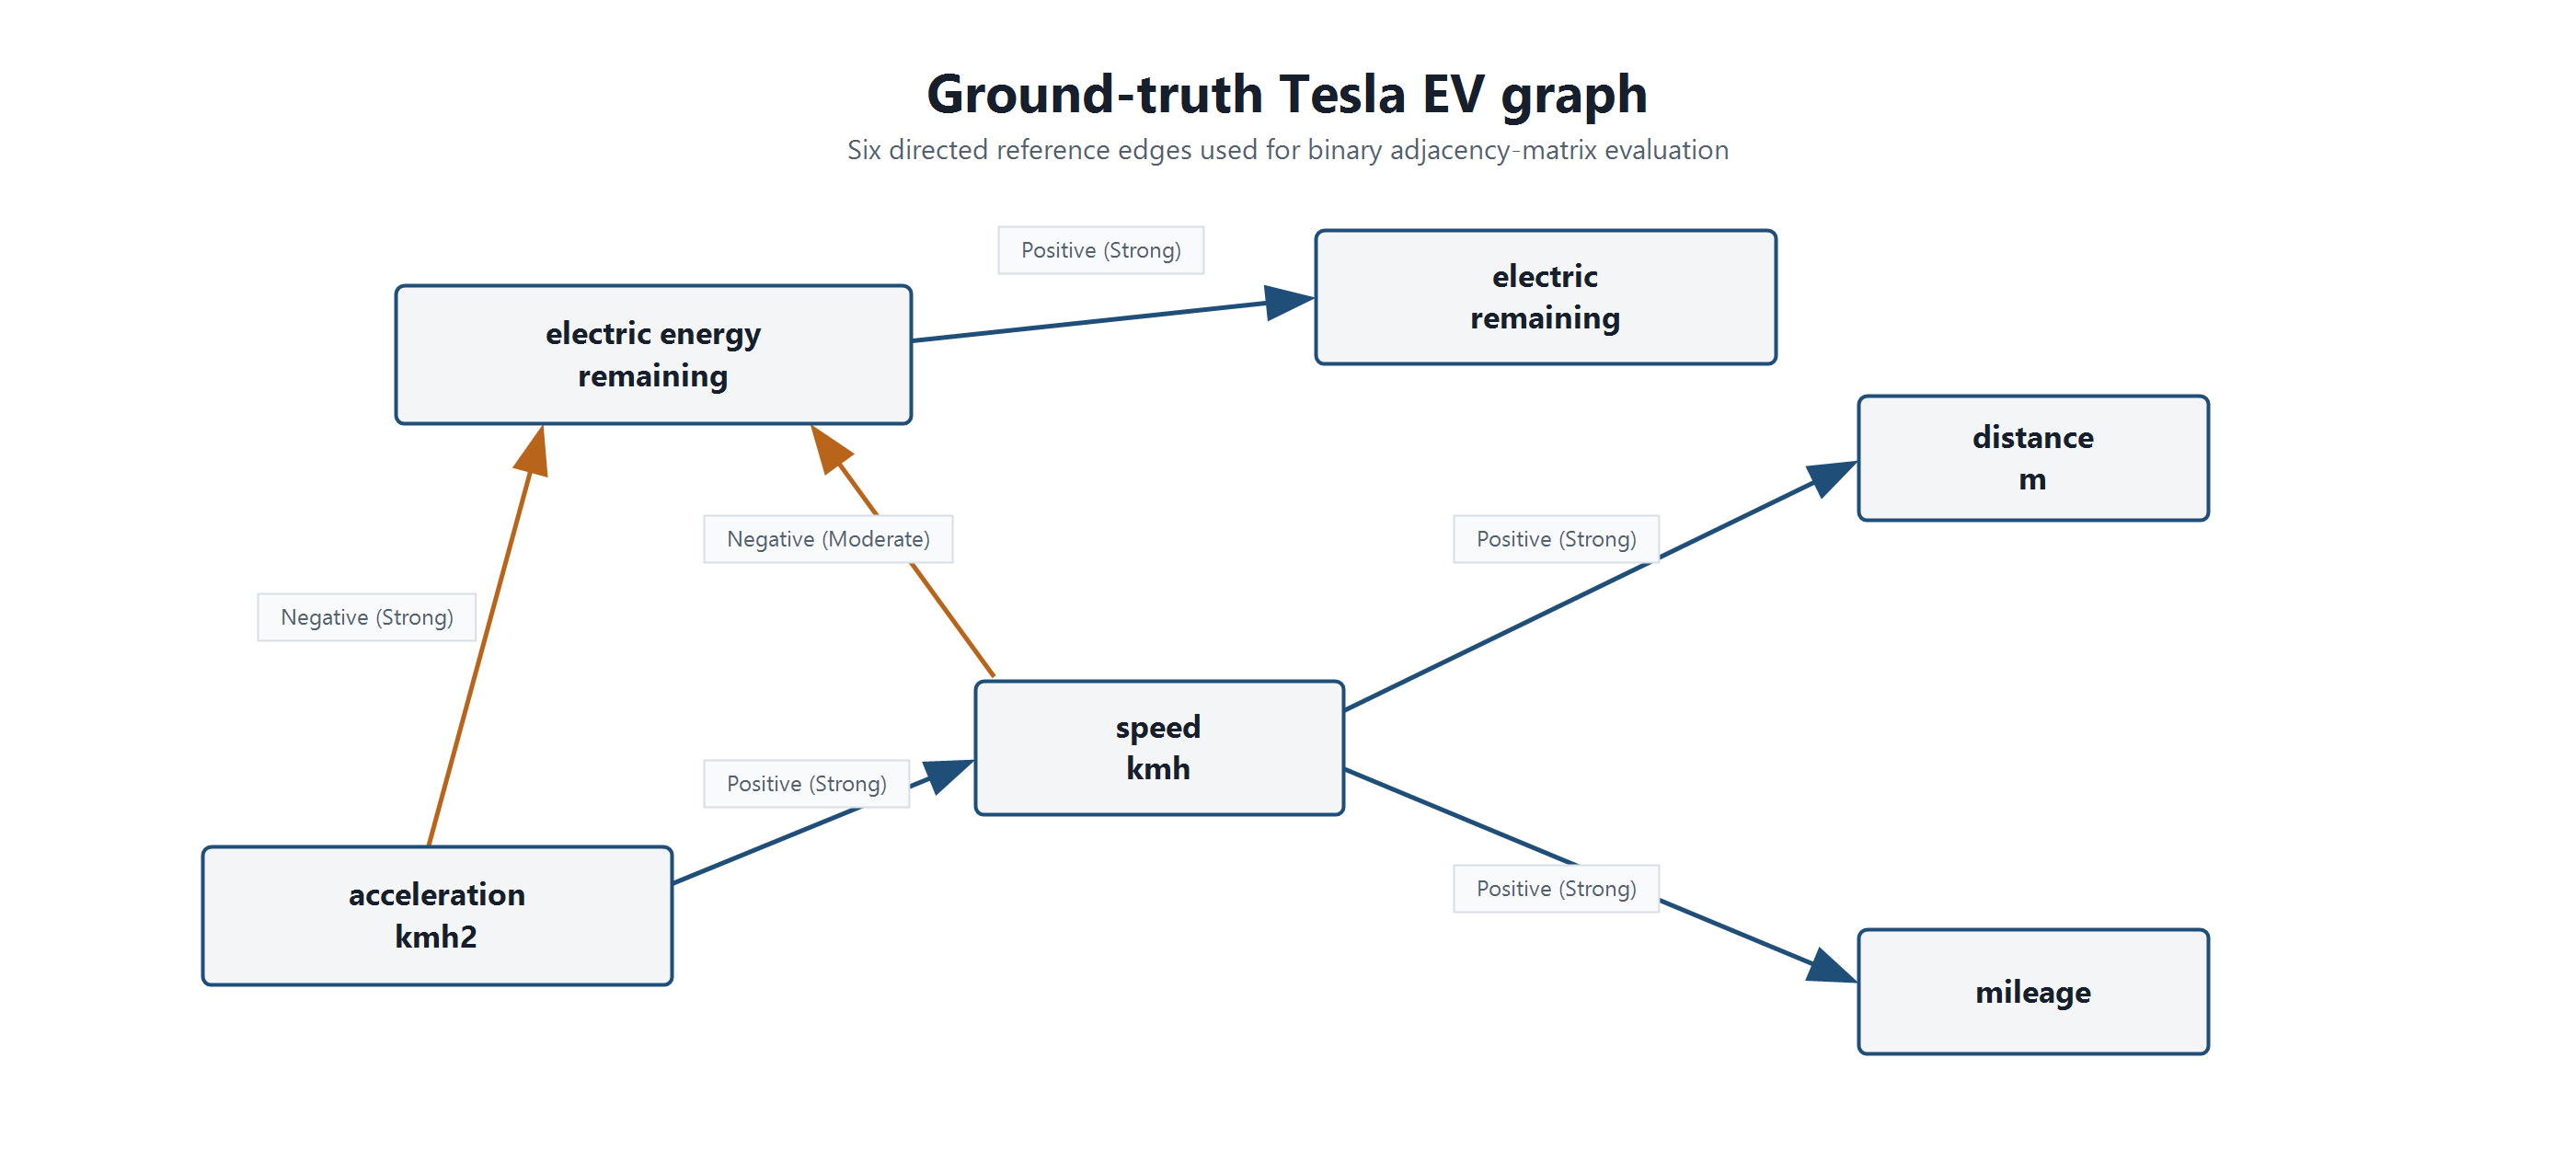
\includegraphics[width=0.86\textwidth]{figures/Ground_Truth_UC_Tesla_Energy_Consumption.png}%
  }{%
    \fbox{\parbox{0.82\textwidth}{Ground-truth DAG image not found. The edge list is shown in Table~\ref{tab:ground-truth-edges}.}}%
  }
  \caption{Ground-truth Tesla EV graph used as the evaluation target. The figure corresponds to the edge list in Table~\ref{tab:ground-truth-edges}.}
  \label{fig:ground-truth-dag}
\end{figure}

\section{Scope and Boundaries}

The graph-recovery task has three boundaries. First, it is single-dataset: all
primary results use the Tesla EV use case. Second, it is prompt-based: the
models are not fine-tuned and no external tool is called during generation.
Third, it is single-output per evaluated cell in the supplied artifacts: the
sidecar JSON files report \texttt{n\_runs = 1}. The notebook contains
repeated-run and self-consistency machinery, but the primary result directory
used in this thesis does not provide executed repeated-run evidence.

Earlier governance-oriented infrastructure remains relevant as supplementary
context. It motivated careful treatment of telemetry fields and local
inference, while the main chapters evaluate graph-recovery performance rather
than disclosure or utility trade-off metrics.
